\documentclass[lettersize,journal]{IEEEtran}
\usepackage{hyperref}
\usepackage{amsmath,amsfonts}
\usepackage{algorithmic}
\usepackage{algorithm}
\usepackage{array}
\usepackage[caption=false,font=normalsize,labelfont=sf,textfont=sf]{subfig}
\usepackage{textcomp}
\usepackage{stfloats}
\usepackage{url}
\usepackage{verbatim}
\usepackage{graphicx}
\usepackage{cite}
\hyphenation{op-tical net-works semi-conduc-tor IEEE-Xplore}
% updated with editorial comments 8/9/2021

\begin{document}

\title{Post Delivery Robot with Deep Q-Learning}

\author{Mohamad Ali Saber\\ \href{mailto:malisaber@yahoo.com}{malisaber@yahoo.com}}


% The paper headers
%\markboth{Journal of Something,~Vol.~14, No.~8, August~2021}%
%{Shell \MakeLowercase{\textit{et al.}}: A Sample Article Using IEEEtran.cls for IEEE Journals}

%\IEEEpubid{0000--0000/00\$00.00~\copyright~2021 IEEE}
% Remember, if you use this you must call \IEEEpubidadjcol in the second
% column for its text to clear the IEEEpubid mark.

\maketitle






\begin{abstract}
In this project, we explore a new area of the Reinforcement Learning (RL) which is application of Function Approximation and Neural Network in the RL. According to the script, the agent learned to pick a postal package from a predefined location and deliver it to another predefined destination within a 5X5 grid-world environment. While the agent is moving within the world, it learned to avoid the obstacles of the map.
Results show that the implemented neural network successfully learned to perform the best action in each situation during the delivery. Also it shows a promising future for application of neural network in the RL problems.
\end{abstract}

\begin{IEEEkeywords}
Reinforcement Learning, Function Approximation, Deep Q-Learning, Neural Network, Post Delivery Robot.
\end{IEEEkeywords}




%%%%%%%%%%%%%%%%%%%%%%%%%%%%%%%%%%%%%%%%%%%%%%%%%%%%%%%%%%%%%%%%%%%%%%%%%%%%%%%%%%
%                   INTERODUCTION
%%%%%%%%%%%%%%%%%%%%%%%%%%%%%%%%%%%%%%%%%%%%%%%%%%%%%%%%%%%%%%%%%%%%%%%%%%%%%%%%%%
\section{Introduction}
\IEEEPARstart{T}{abular} Reinforcement Learning methods have a critical limitation, as their state size growth, their computational complexity grows exponentially. This exponentially growth rate makes tabular-based methods to struggle to converge to a optimum solution. Another problem with the tabular methods is that many of real-world's problems cannot be presented using tables; as the result, a non-tabular based method is most needed.\par

Function Approximation helps us to migrate from the conventional tabular Reinforcement Learning Methods to non-tabular method. Function Approximation utilize various type of function to approximate the action-value calculation. One of its widely use approximations is Neural Network, in which an artificial intelligence (in here, a multi-layer fully-connected network) estimates the value for each action based on the present state of the agent. At the end, this AI replaces the action-value table and acts as the brain of the agent.\par

In contrary to the conventional MLP applications, which supervisely train on an static data set, those that are used in the RL scenarios do not have pre-defined labeled data and should be learned differently. Another difference is that the Neural Network in RL applications should be learned on non-static data. Despite these difficulties, NNs show promising capability in approximating the action-value function.\par

In this project, the power of a MLP network with one hidden layer consisting of 128 neurons will be exploited. The implemented neural network takes the state as a one-hot vector of 500 different states and generates action values of all possible action in that states. Then, the agents choose the best action based on its value.\par

The rest of this report organizes as:
\begin{itemize}
    \item Section II: Methodology
    \item Section III: a brief explanation of the implemented code
    \item Section IV: Training, simulation and results
    \item Section V: Conclusion
\end{itemize}
\vspace{0.3cm}


%%%%%%%%%%%%%%%%%%%%%%%%%%%%%%%%%%%%%%%%%%%%%%%%%%%%%%%%%%%%%%%%%%%%%%%%%%%%%%%%%%
%                   Methodology
%%%%%%%%%%%%%%%%%%%%%%%%%%%%%%%%%%%%%%%%%%%%%%%%%%%%%%%%%%%%%%%%%%%%%%%%%%%%%%%%%%
\section{Methodology}
In this section, the environment and its setup, states, and actions will be discussed firstly, then the reward function will be presented. After that, the architecture of Neural Network will explored, and lastly, the training process and hyper parameters will be discussed.

    \subsection{Environment}
    A MATLAB class were developed to mimic the dynamics of the environment and provides essential method function trough the learning process. This class simulate a 5X5 grid-world environment which presented in the project script with same boundaries, obstacles, and packet as well as destination locations. A car can move freely within the map and performs one of considered actions at a time step. \par

    The state action of the environment is a quadruplet consists of latitude and longitude of car position, an index denoting the destination, and another index to indicate the location of package. Since the agent is living within a 5X5 grid-word, its latitude and longitude can be number between 0 to 4, 4 possible destination suggests that its index should be from 1 to 4. Lastly, the package index should cover 4 possible location of package, as well as when the car picks the package; as a result, it should be in range of 1 to 5. In conclusion, the agent can experience $5 \times 5 \times 4 \times 5 = 500$ different states.\par

    In each state, the agent can perform 4 possible movement to the North, East, South, and West location. Along with this action, it can also pick the package or drop it; which leading to a 6 possible actions in each state.\par

    Some actions are illegal in a certain states, for example dropping the package in any location except the destination is illegal, also picking a package in a wrong place is illegal. Beside that, the agent is prohibited from leaving the map and any attempt to leave the map is illegal. Lastly, hitting the walls within the map is illegal too. Each illegal move leading to receiving reward of -10 in that move. Successfully drop the package at the destination cause a positive reward equal to 20. Any move except above mentioned cause receiving a -1 reward in each steps. The received reward can be formulate as bellow.\par
    
    \begin{equation}
    R = -1 - 9*illegal + 21 * success
    \end{equation}
    
    
    
    \subsection{Neural Network}
    The implemented neural network is a simple MLP with one hidden layer consist of 128 neurons with ReLu activation function. The network takes a one-hot vector with length of 500 which the hot one is corresponded to the state of the agent. In the output, it generates a 6D vector of action values each one corresponded to value of one action in the given state. The figure \ref{fig:net} shows the architecture of the implemented neural network.\par
    
    \begin{figure}
        \centering
        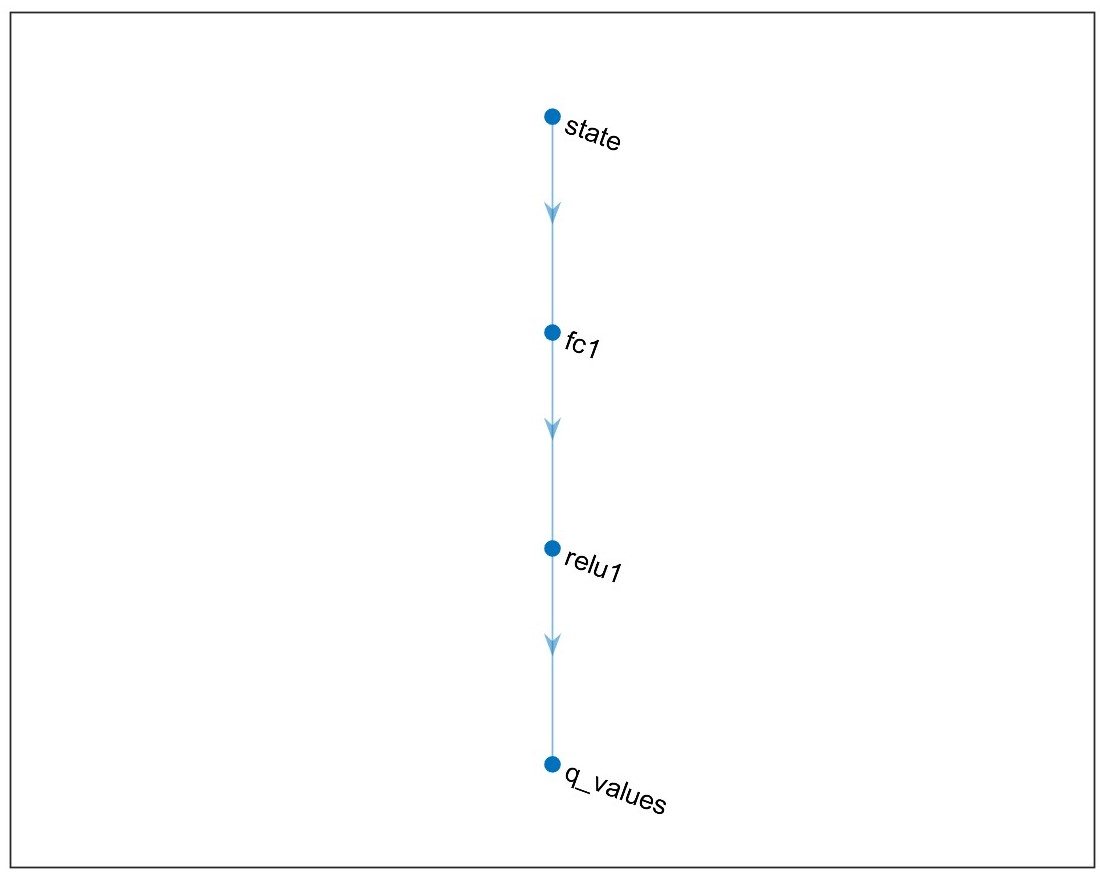
\includegraphics[width=0.9\linewidth]{pics/net.jpg}
        \caption{\centering Architecture of implemented Neural Network}
        \label{fig:net}
    \end{figure}
    
    
    
    \subsection{Training Process}
    The Deep Q-Learning (DQN) algorithm starts with hyperparameter with the exact value as mentioned in the script. To be precise, the learning continues for 10,000 episodes, in each, the agent interacts with the environment in order to successfully deliver the package or the episode terminate after 100 steps. The agent has the discount factor of 0.99. The DQN algorithm utilize a reply buffer with size of 50,000 which stores past 50,000 transition of the agent within the environment. Each row is a quintuplet vector consists of a single transaction information in the format of (Present State, Action, Reward, Next State, Is Done?). This buffer fills once at the beginning of the training process and each row replaces and updates consecutively in each state of each episode. \par
    
    At each step of each episode, the Neural Network of DQN algorithm learns on a batch of input data which fetch randomly from the entire reply buffer. During the training process, the batch size is constant and equal to 32. To achieve a smooth learning process the learning rate chosen to be 0.00025 at the beginning of the process and decay gradually after each 10,000 training steps. The formula used to resemble the decay is below. \par
    
    \begin{equation}
    epsilon = \frac{epsilon_{base}}{1 + 0.1 \times [\frac{iter}{10,000}]}
    \end{equation}
    
    The agent uses $\epsilon$-greedy policy with respect to the action-value of each action in the given state. The agent need to explore all possible actions in each states in the beginning of the learning process, when it explores enough, it should exploit its knowledge to chose the best action and updates its estimation of action-values. To achieve so and also smooth transition from exploring to exploiting, the start value of $\epsilon$ was set to 1 and it decays geometrically after each episode with factor of 0.999 which indicates that at the end of learning process, value of the epsilon reaches to 0.00004. It is worth mentioning that the target model updates after each 100 training steps. It is worth mentioning that initially, the neural network used stochastic gradient decent to update the learnable weight of the network, but after a trial run, I decided to use the Adam optimizer for its faster and smother convergence.
    

%%%%%%%%%%%%%%%%%%%%%%%%%%%%%%%%%%%%%%%%%%%%%%%%%%%%%%%%%%%%%%%%%%%%%%%%%%%%%%%%%%
%                   Simulation and results
%%%%%%%%%%%%%%%%%%%%%%%%%%%%%%%%%%%%%%%%%%%%%%%%%%%%%%%%%%%%%%%%%%%%%%%%%%%%%%%%%%
\section{Training, Simulation and results}
During Training, at each episode, the loss and average reward of that episode stores in a separate arrays, and at the end of each episode, the trained network evaluates for 8 different scenarios and the average reward and average loss stores separately. Plotting this information during the training process helps us to supervise the learning and detect any abnormality in their behaviours; as a result, changing the hyper parameters. Beside the training and validation loss and average reward, the average episode length is also plotted, this information helps the supervisor to track the effectiveness of learning process. As depicted in the figure \ref{fig:progress}, the learning process took 12 hour to complete (The image shows 19 hour because I paused the process for 7 hour so I go to sleep). The above mentioned figure is also depicted the loss and average reward curves for both of training and validation parts. The smoothen curve of average reward in both scenarios is depicted in the figure \ref{fig:smooth}. \par

\begin{figure}
    \centering
    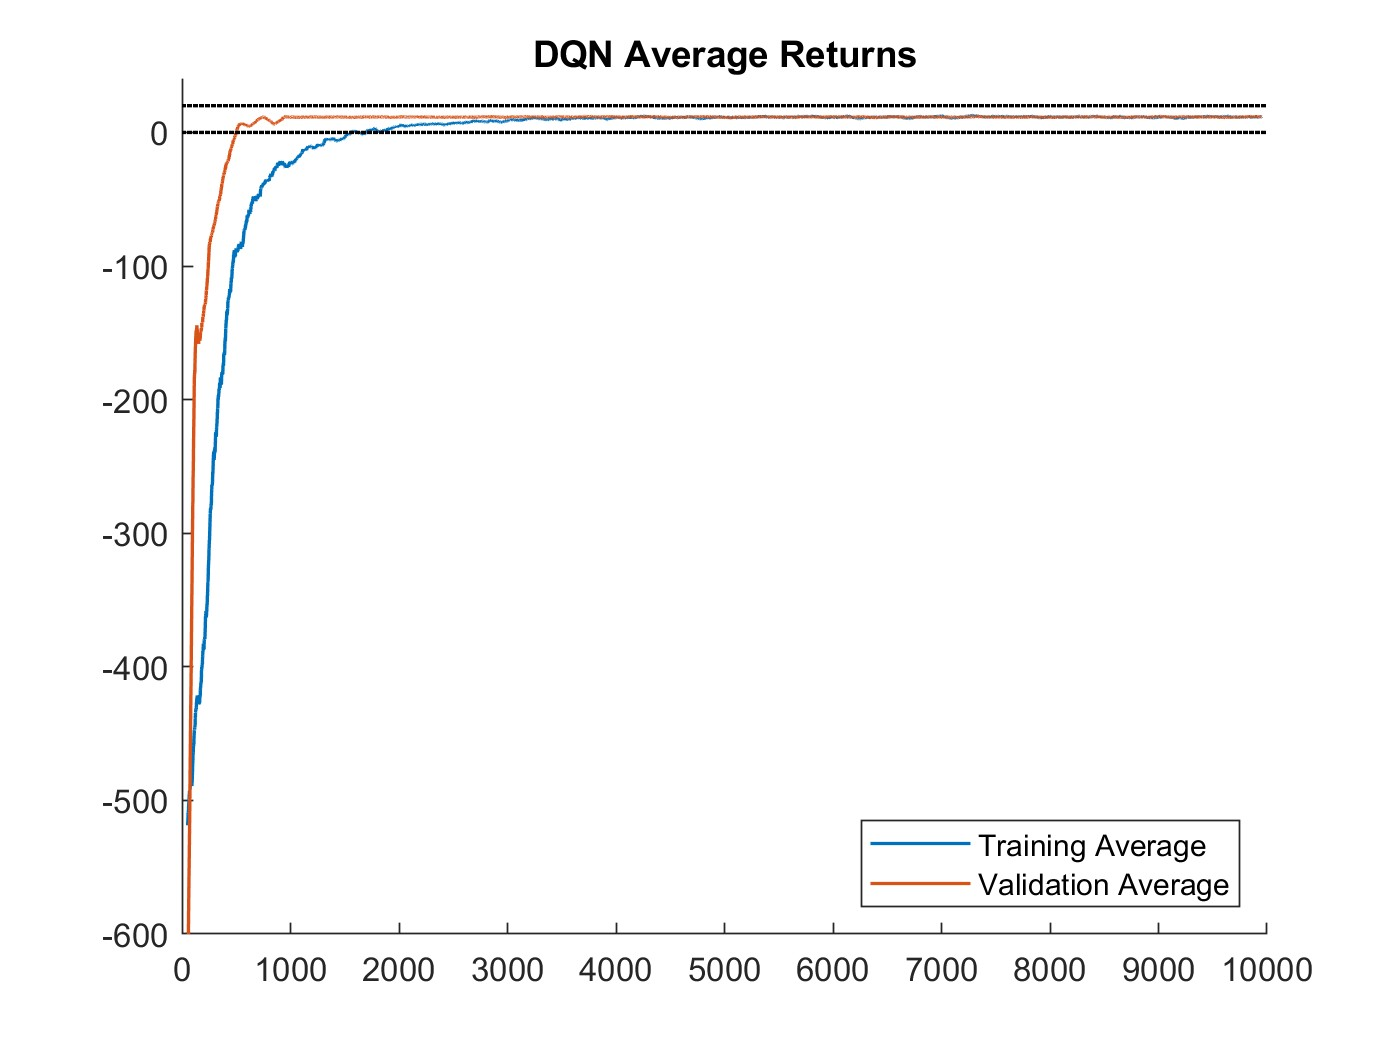
\includegraphics[width=0.9\linewidth]{pics/Ave_ret.jpg}
    \caption{\centering Average reward during the training process smoothen over a 100 window size.}
    \label{fig:smooth}
\end{figure}

\begin{figure*}
    \centering
    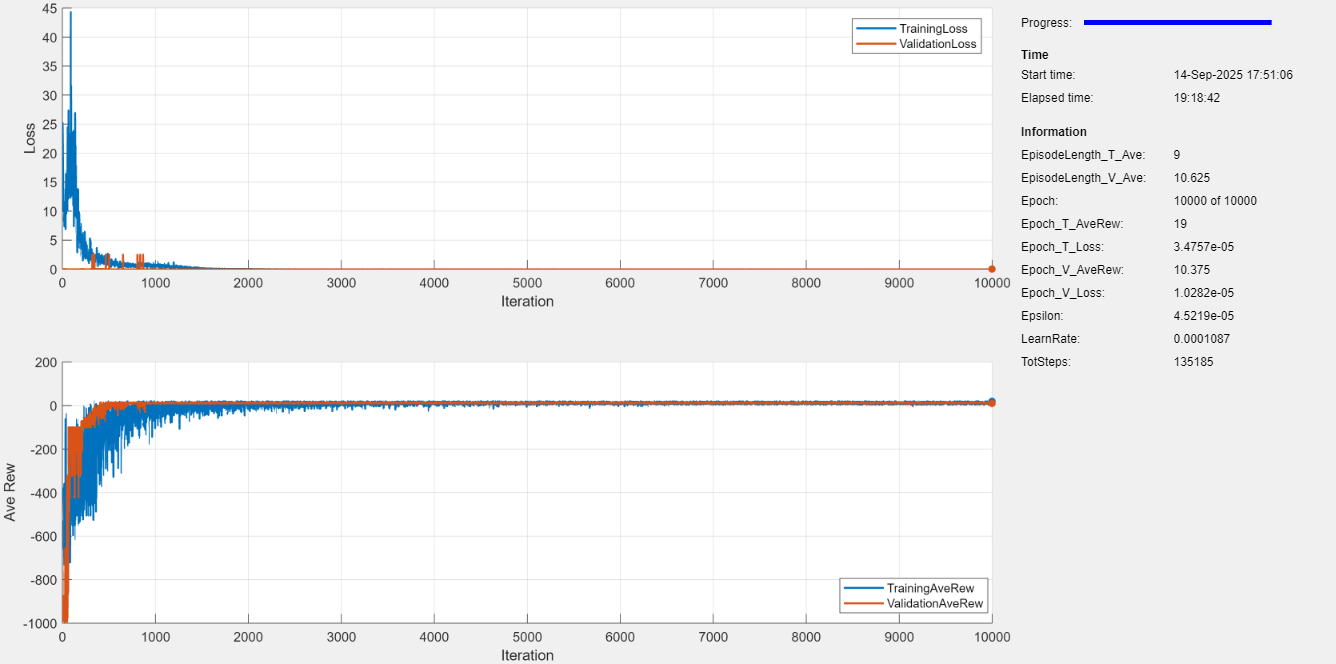
\includegraphics[width=0.9\linewidth]{pics/Progress.PNG}
    \caption{\centering Loss and average reward curves of training and validation scenarios during the training process.}
    \label{fig:progress}
\end{figure*}

The action-value and greedy policy that obtained from the network are depicted in the following. The generated policy by the network is near optimum policy flawlessly, and the action value is also is compatible with the policy and has approximately similar value to those expected. The figure \ref{fig:ANW}-\ref{fig:AWC} shows policy for all 20 different situations of package and the destination location. The state-value of these different situations are depicted in figure \ref{fig:VNW}-\ref{fig:VWC}. 

\begin{figure}
    \centering
    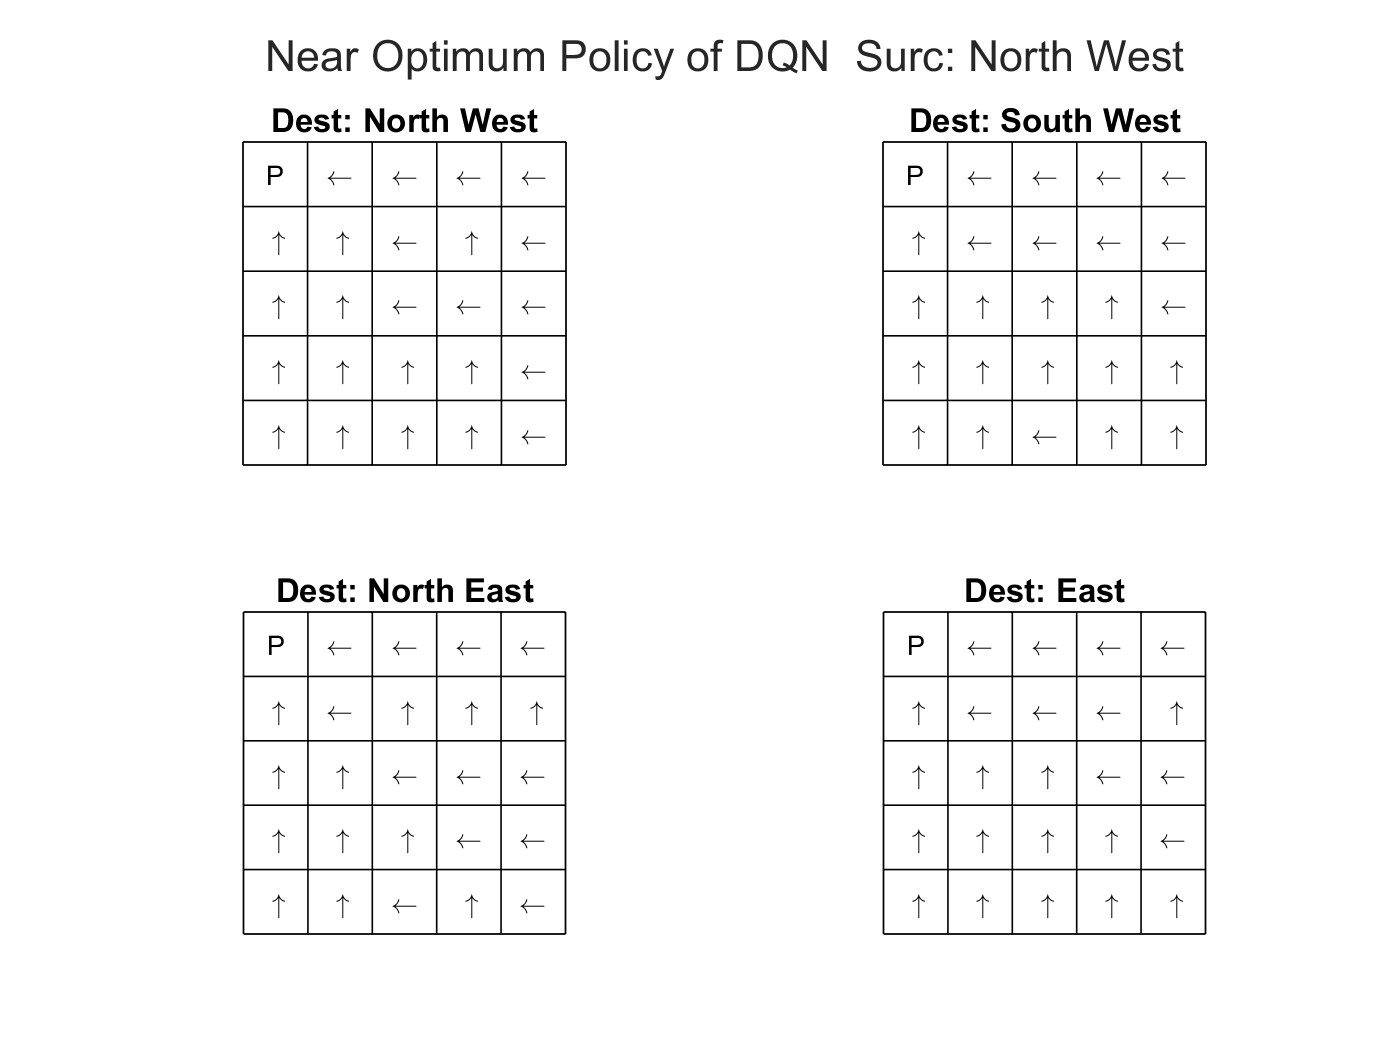
\includegraphics[width=0.9\linewidth]{pics/A_NW.jpg}
    \caption{\centering Agent policy when the package is in the North West of the map for 4 different destinations.}
    \label{fig:ANW}
\end{figure}

\begin{figure}
    \centering
    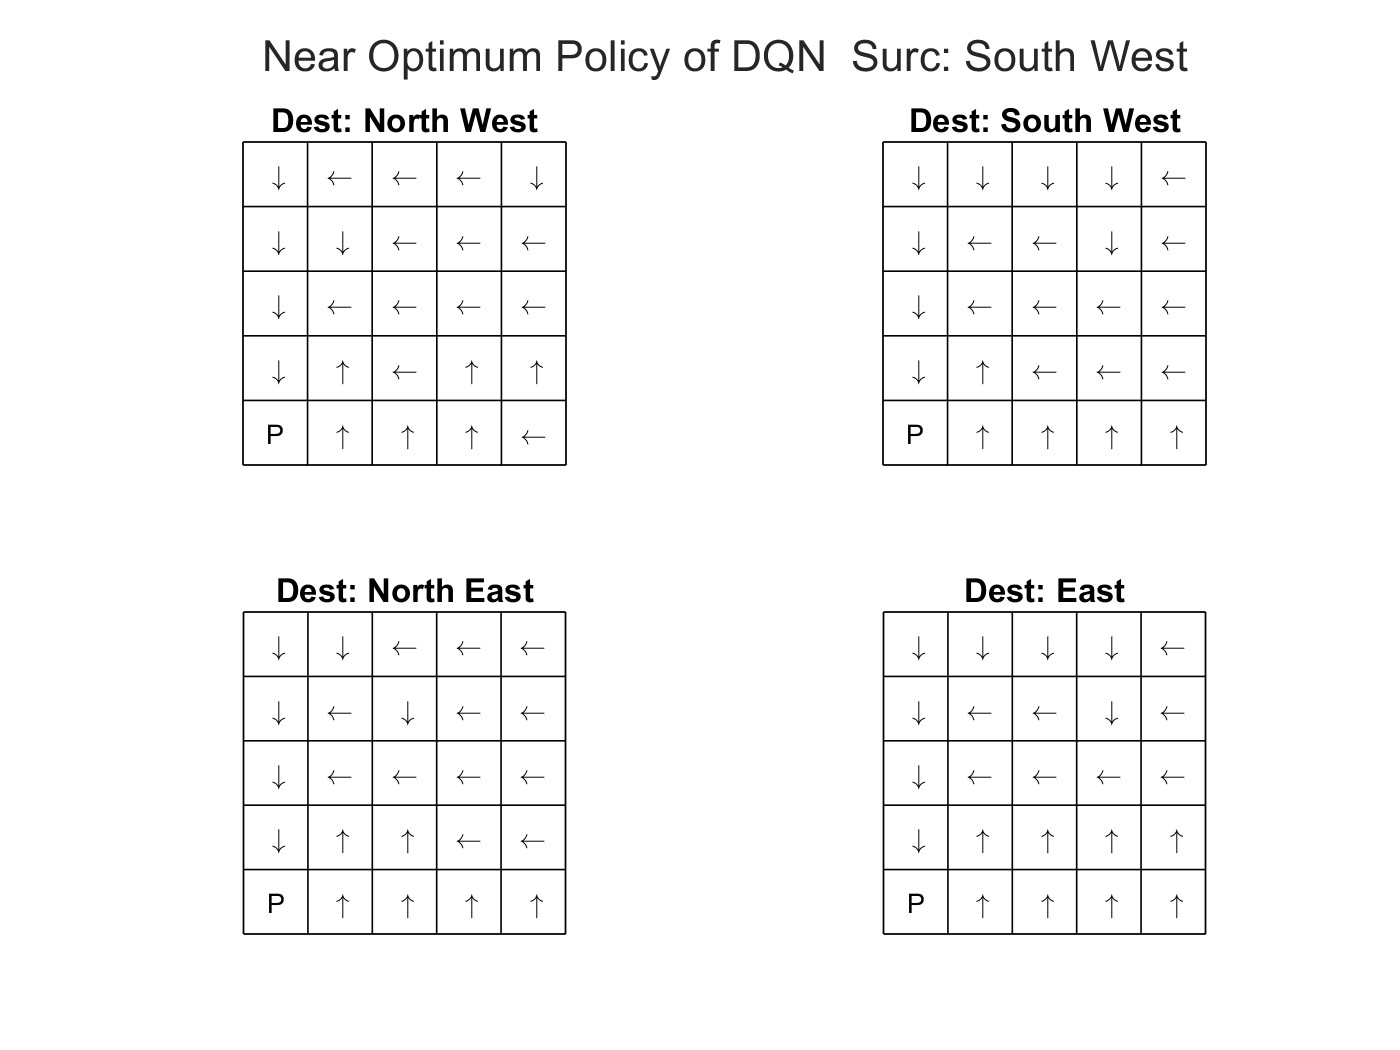
\includegraphics[width=0.9\linewidth]{pics/A_SW.jpg}
    \caption{\centering Agent policy when the package is in the South West of the map for 4 different destinations.}
    \label{fig:ASW}
\end{figure}

\begin{figure}
    \centering
    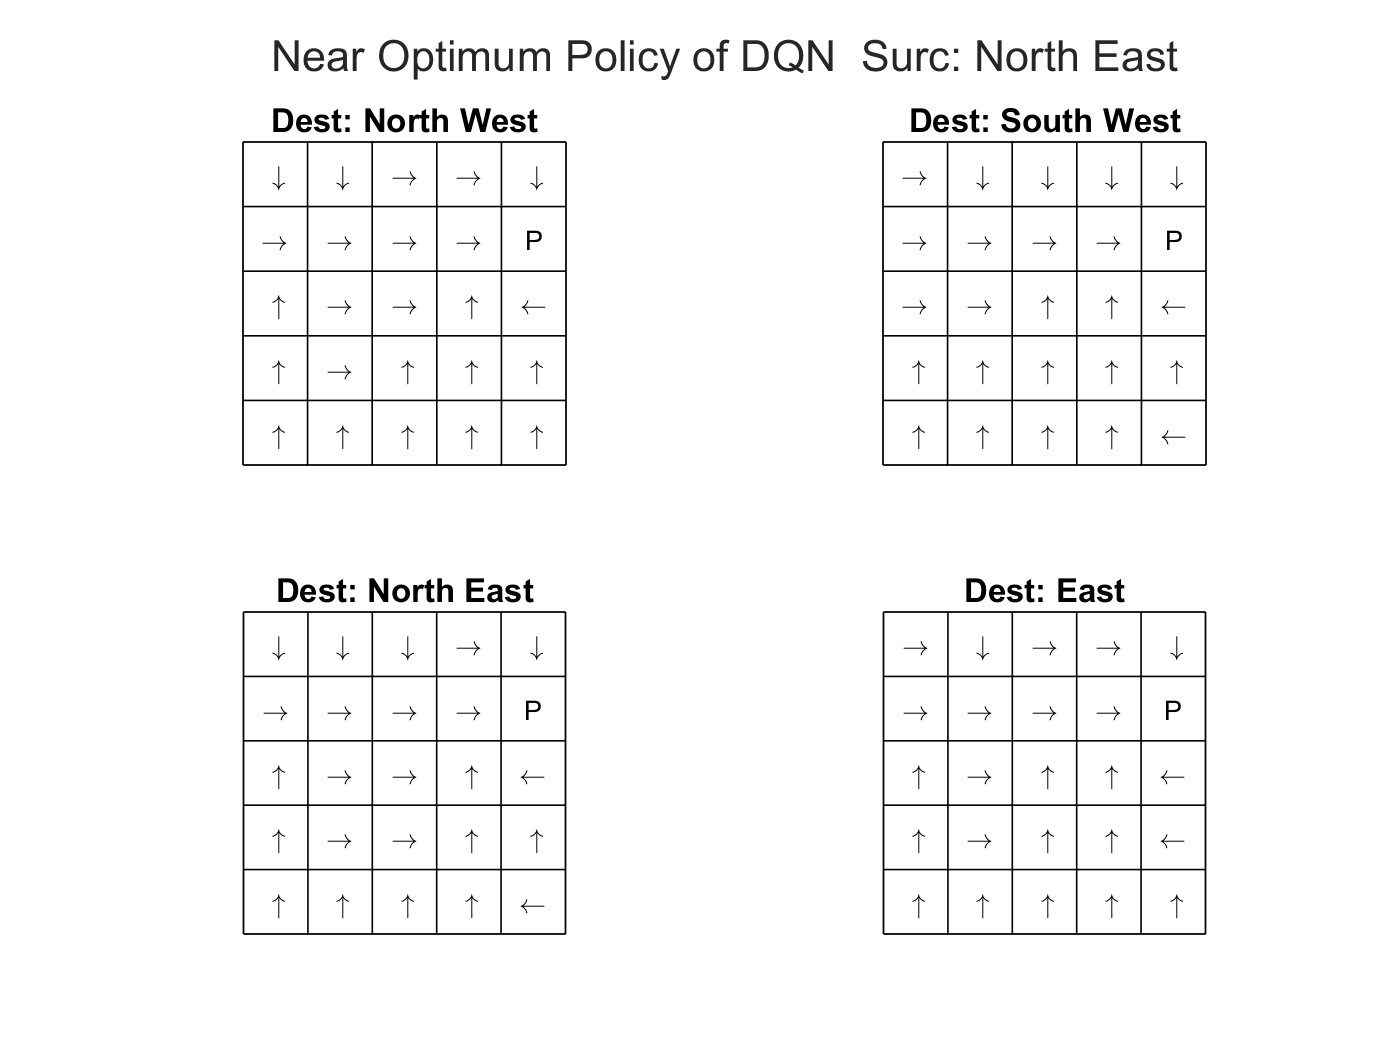
\includegraphics[width=0.9\linewidth]{pics/A_NE.jpg}
    \caption{\centering Agent policy when the package is in the North East of the map for 4 different destinations.}
    \label{fig:ANE}
\end{figure}

\begin{figure}
    \centering
    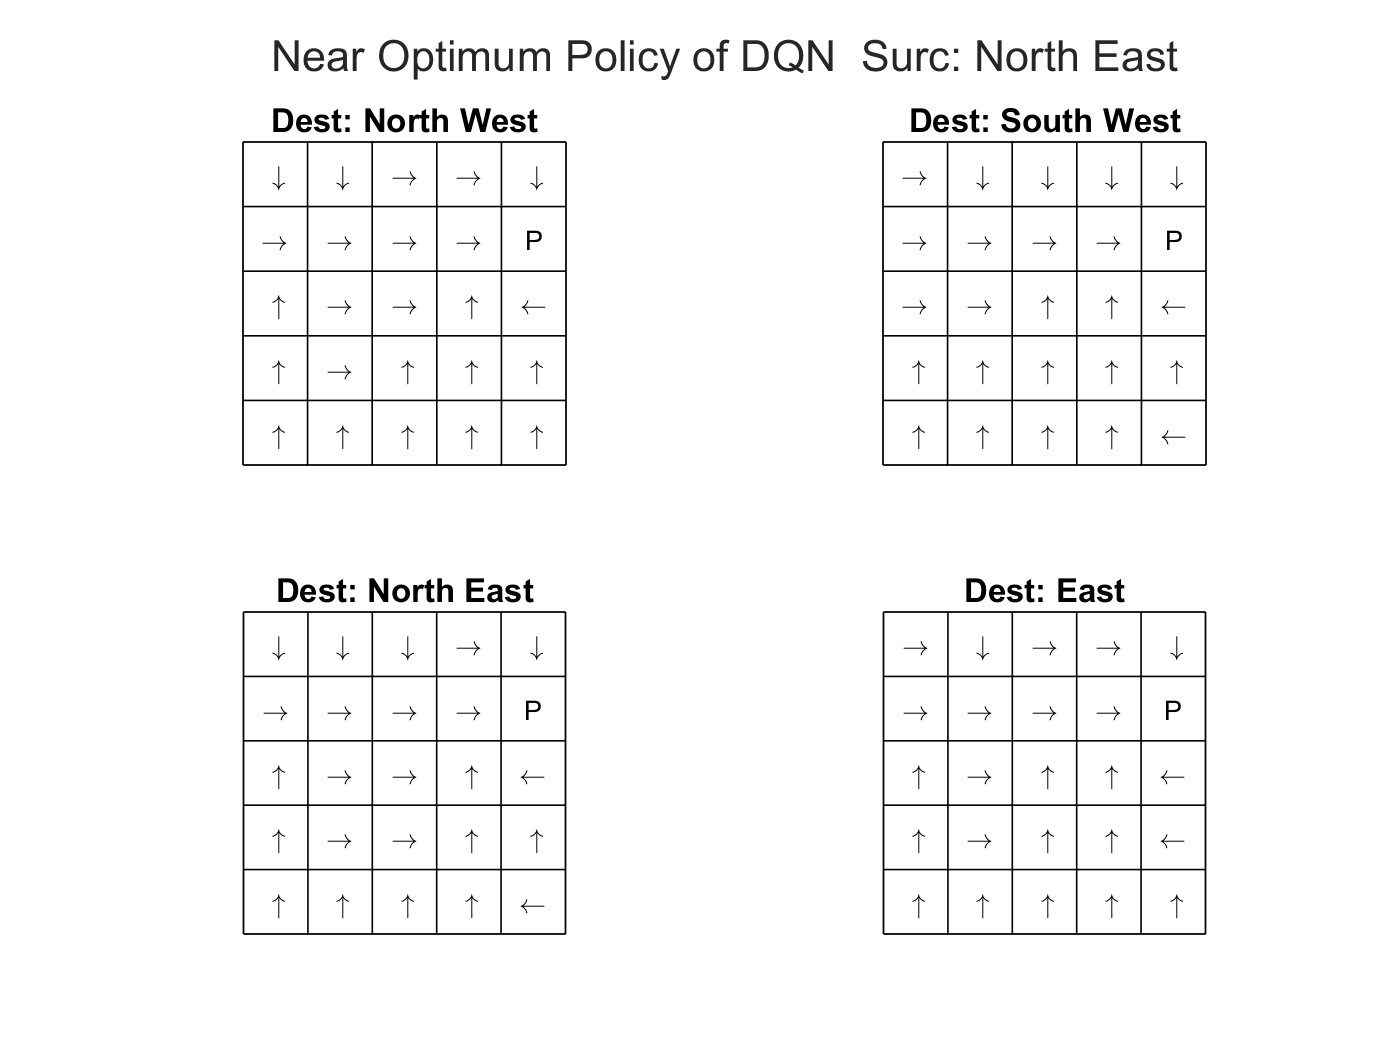
\includegraphics[width=0.9\linewidth]{pics/A_NE.jpg}
    \caption{\centering Agent policy when the package is in the East of the map for 4 different destinations.}
    \label{fig:AE}
\end{figure}

\begin{figure}
    \centering
    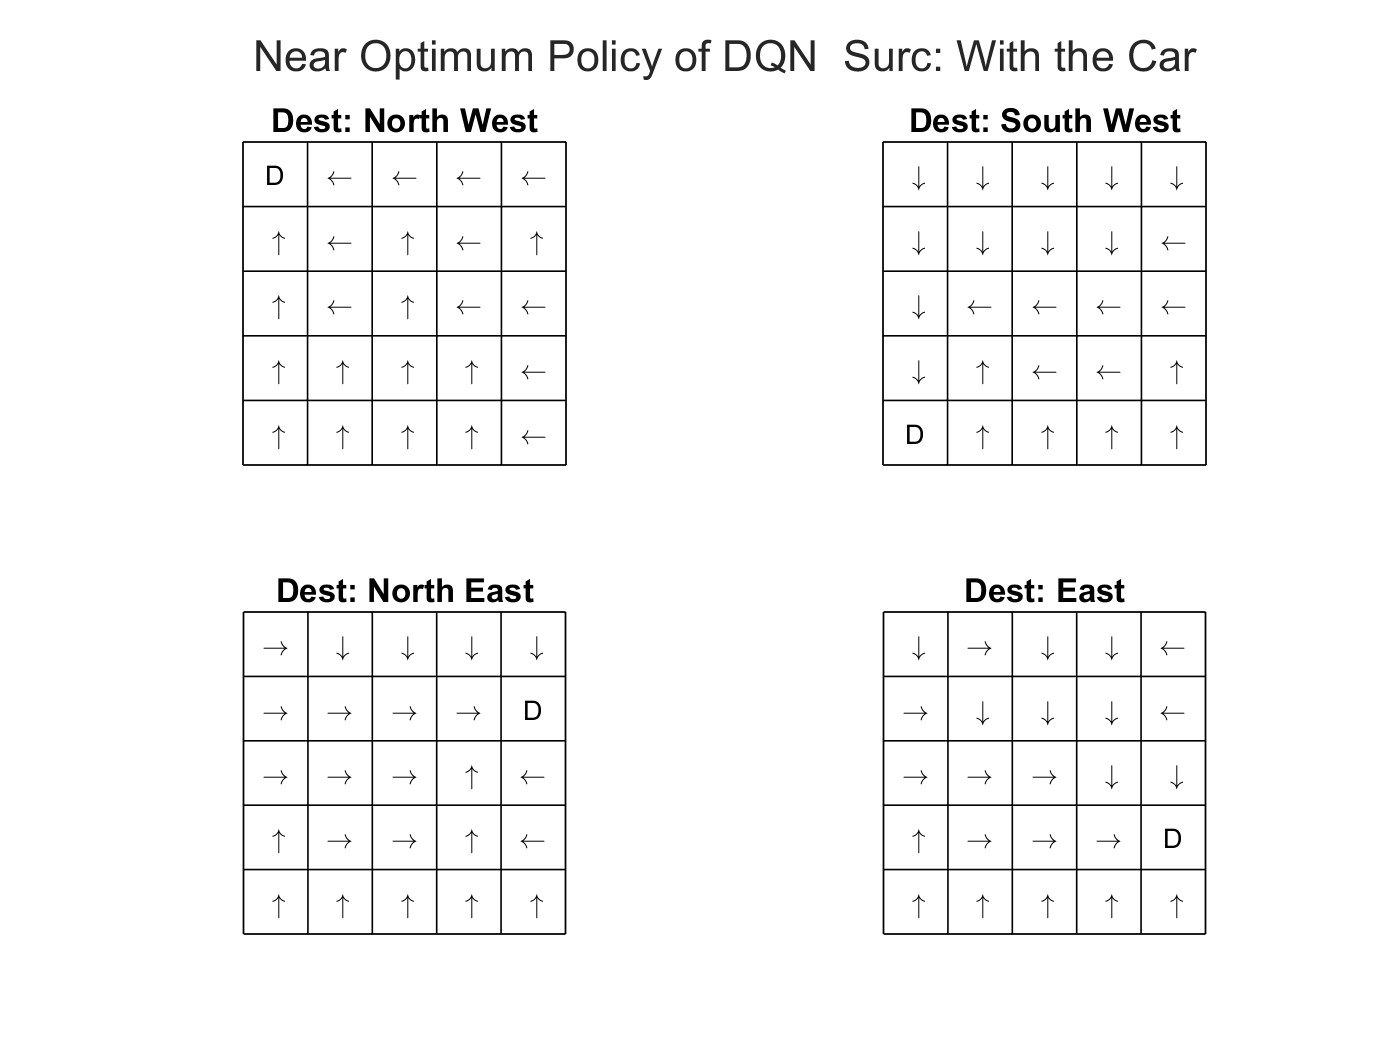
\includegraphics[width=0.9\linewidth]{pics/A_WC.jpg}
    \caption{\centering Agent policy when the package loaded into the car for 4 different destinations.}
    \label{fig:AWC}
\end{figure}





\begin{figure}
    \centering
    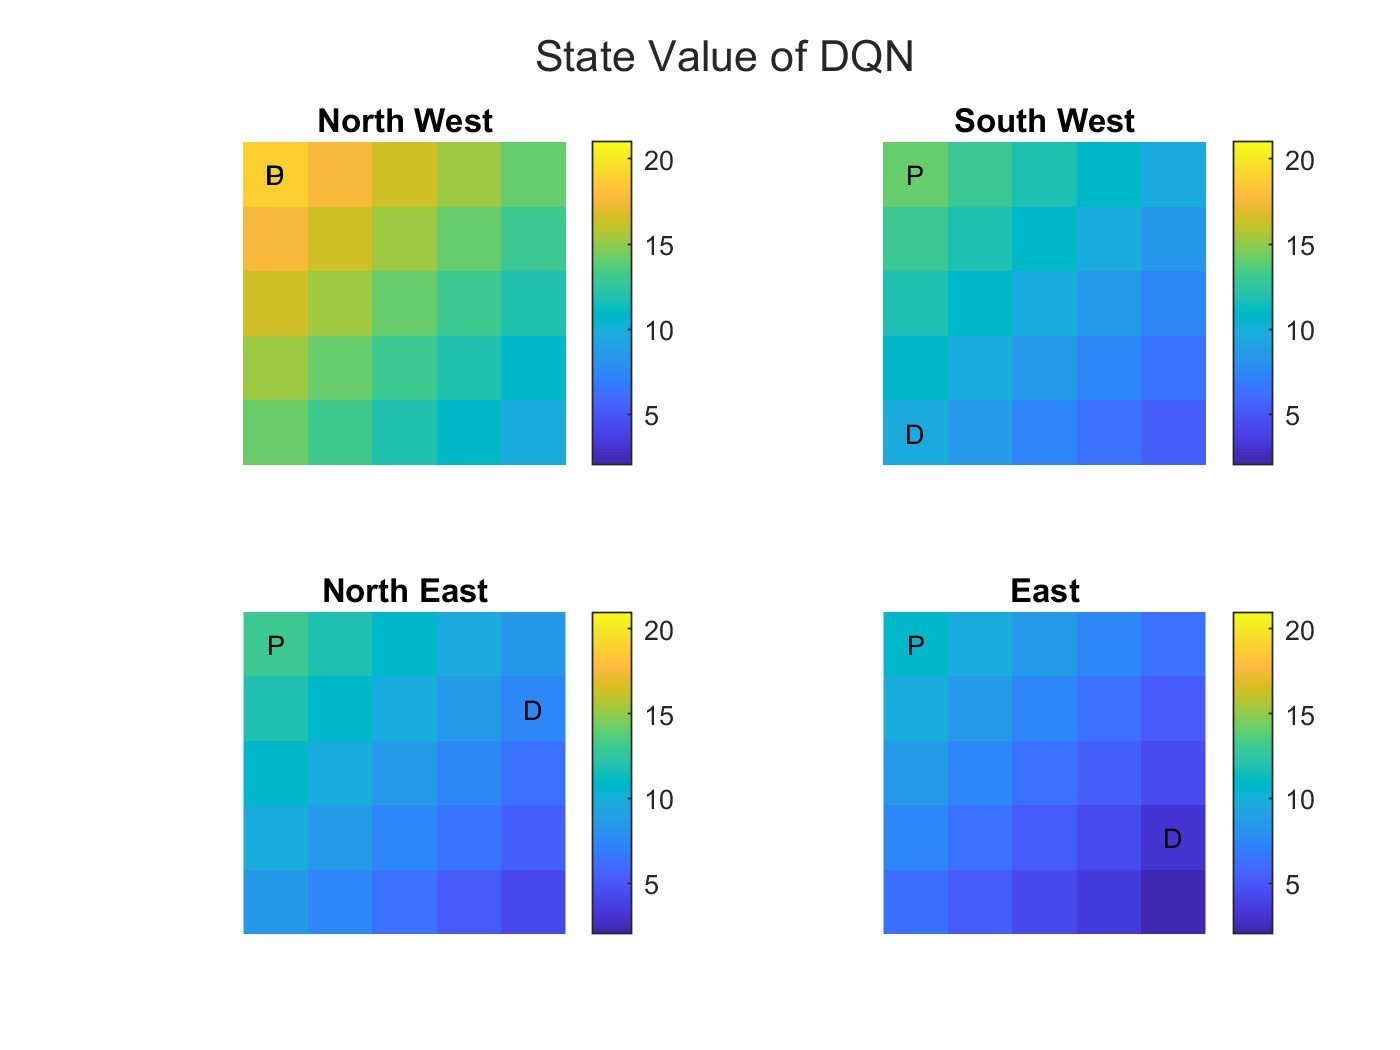
\includegraphics[width=0.9\linewidth]{pics/Vs_NW.jpg}
    \caption{\centering State value of each state when the package is in the North West of the map for 4 different destinations.}
    \label{fig:VNW}
\end{figure}

\begin{figure}
    \centering
    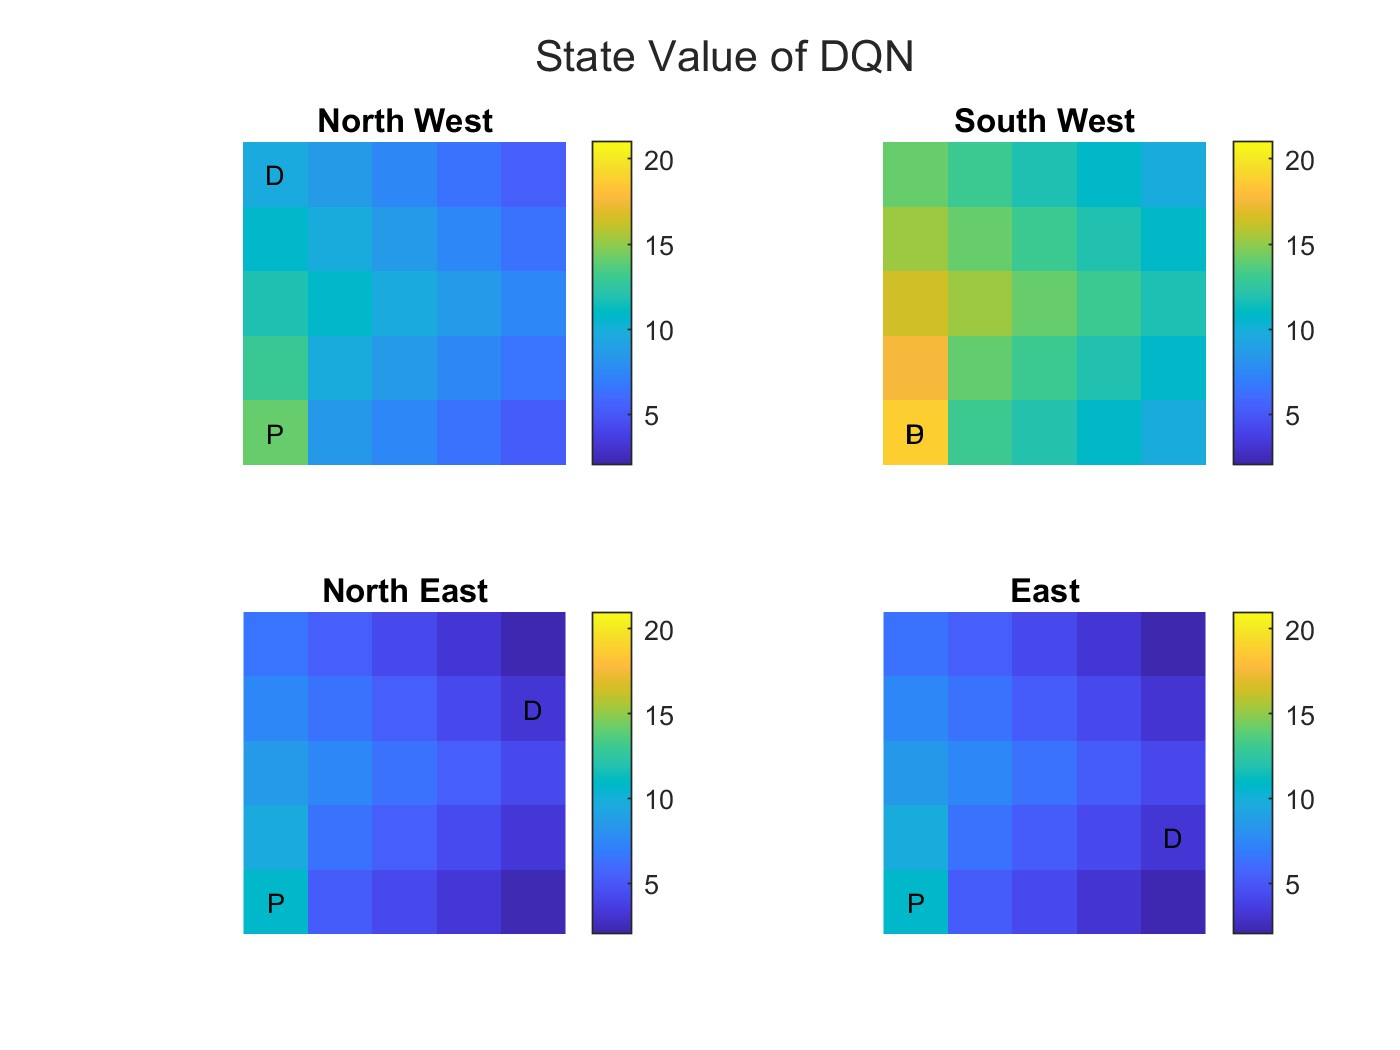
\includegraphics[width=0.9\linewidth]{pics/Vs_SW.jpg}
    \caption{\centering State value of each state when the package is in the South West of the map for 4 different destinations.}
    \label{fig:VSW}
\end{figure}

\begin{figure}
    \centering
    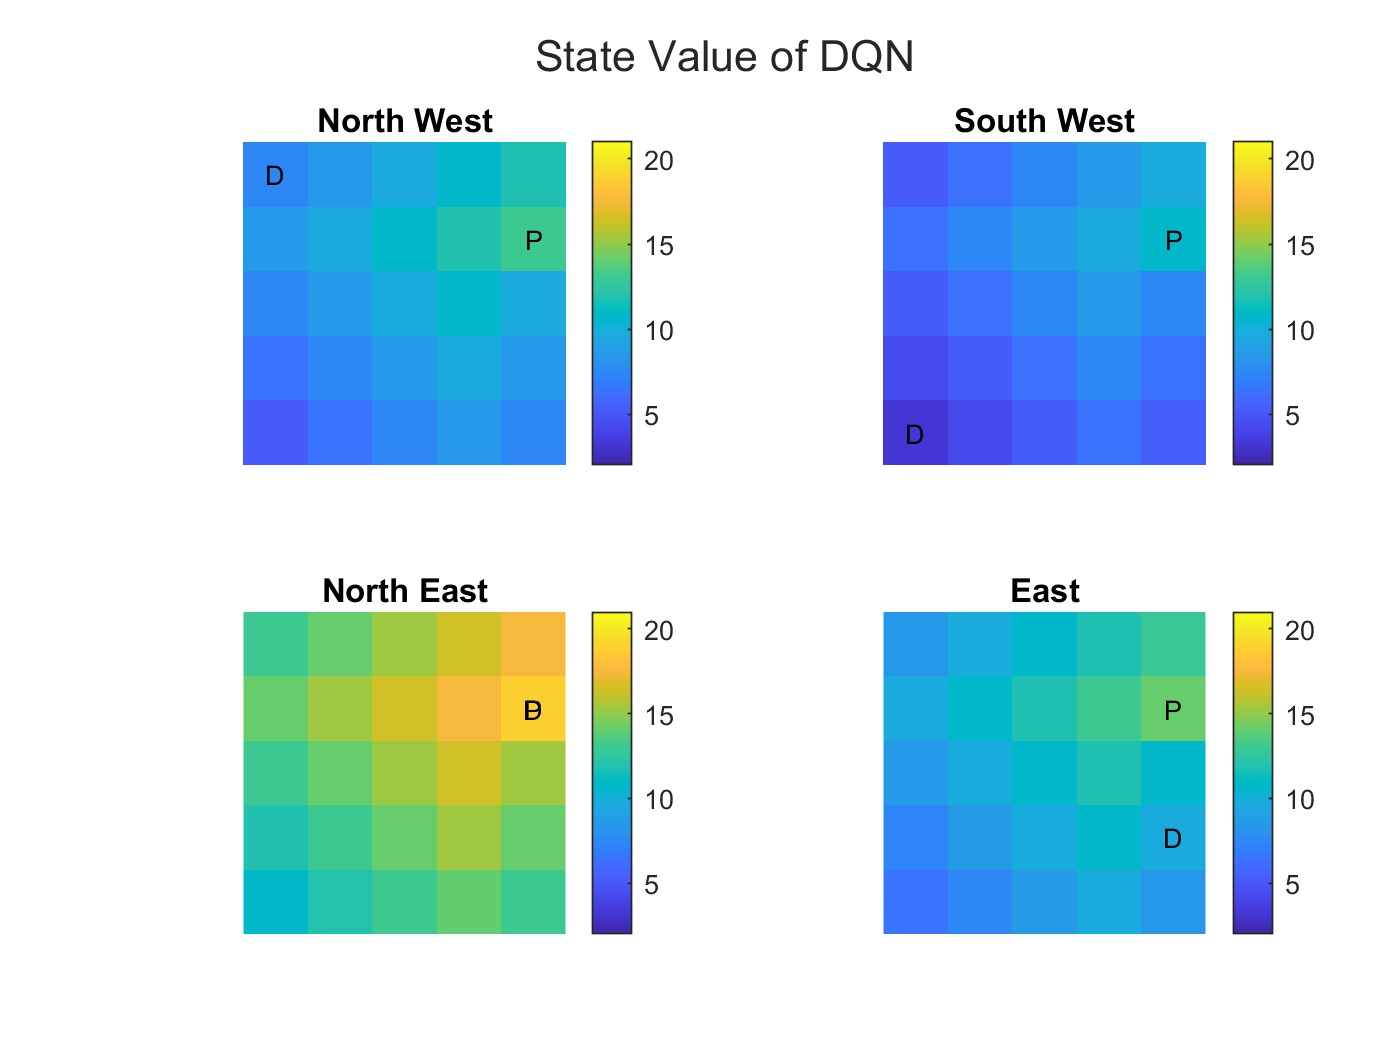
\includegraphics[width=0.9\linewidth]{pics/Vs_NE.jpg}
    \caption{\centering State value of each state when the package is in the North East of the map for 4 different destinations.}
    \label{fig:VNE}
\end{figure}

\begin{figure}
    \centering
    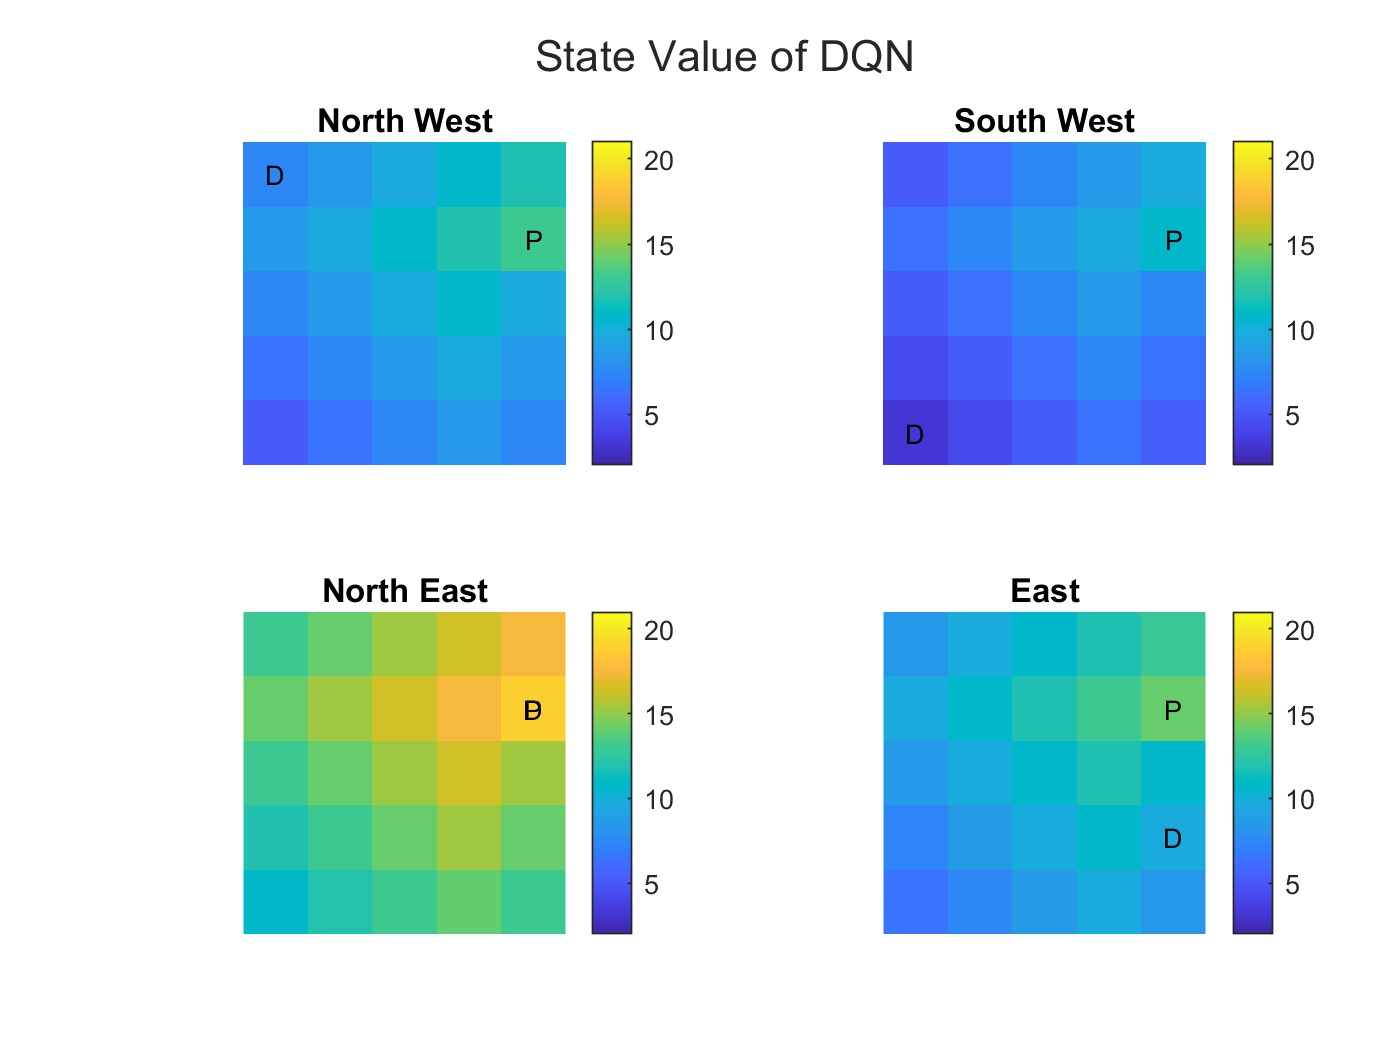
\includegraphics[width=0.9\linewidth]{pics/Vs_NE.jpg}
    \caption{\centering State value of each state when the package is in the East of the map for 4 different destinations.}
    \label{fig:VE}
\end{figure}

\begin{figure}
    \centering
    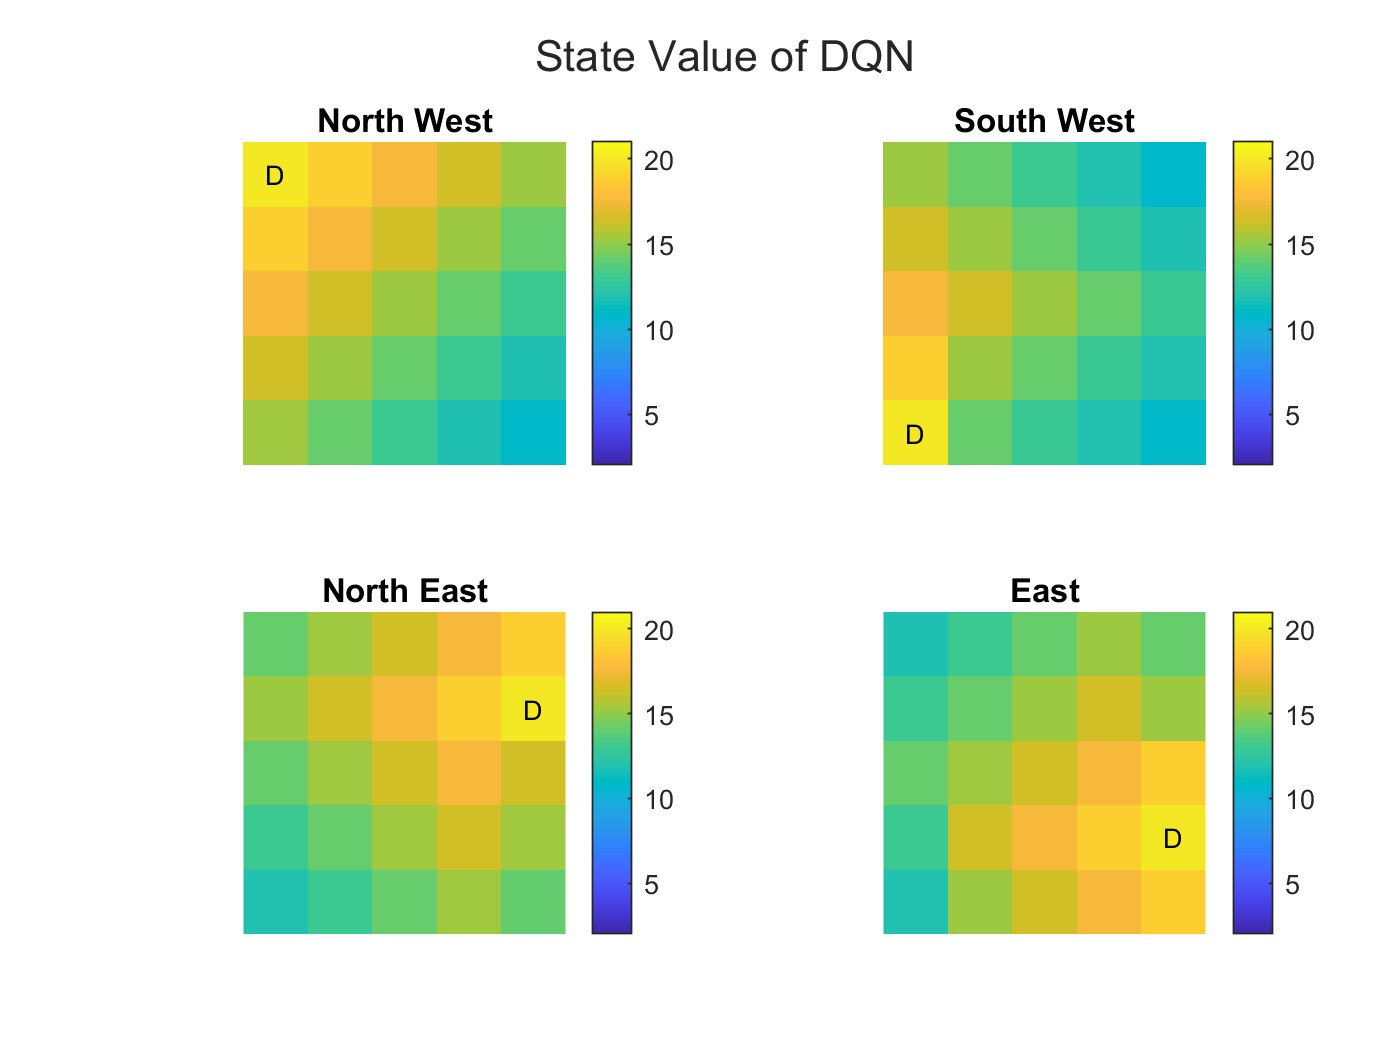
\includegraphics[width=0.9\linewidth]{pics/Vs_WC.jpg}
    \caption{\centering State value of each state when the package loaded into the car for 4 different destinations.}
    \label{fig:VWC}
\end{figure}


The simulation of the environment is also confirms the correctness of learning process. The figure \ref{fig:SIM} shows the simulation of an episode; in which, the agent respawn at the south west of the map, the destination is right above it at the north west corner, but the package is at the east. At first, it went to the location of the package, then picked it up, and delivered it to the destination; as a result, receiving total reward of 6.14 upon the completion of episode.

\begin{figure*}
    \centering
    \subfloat[]{
        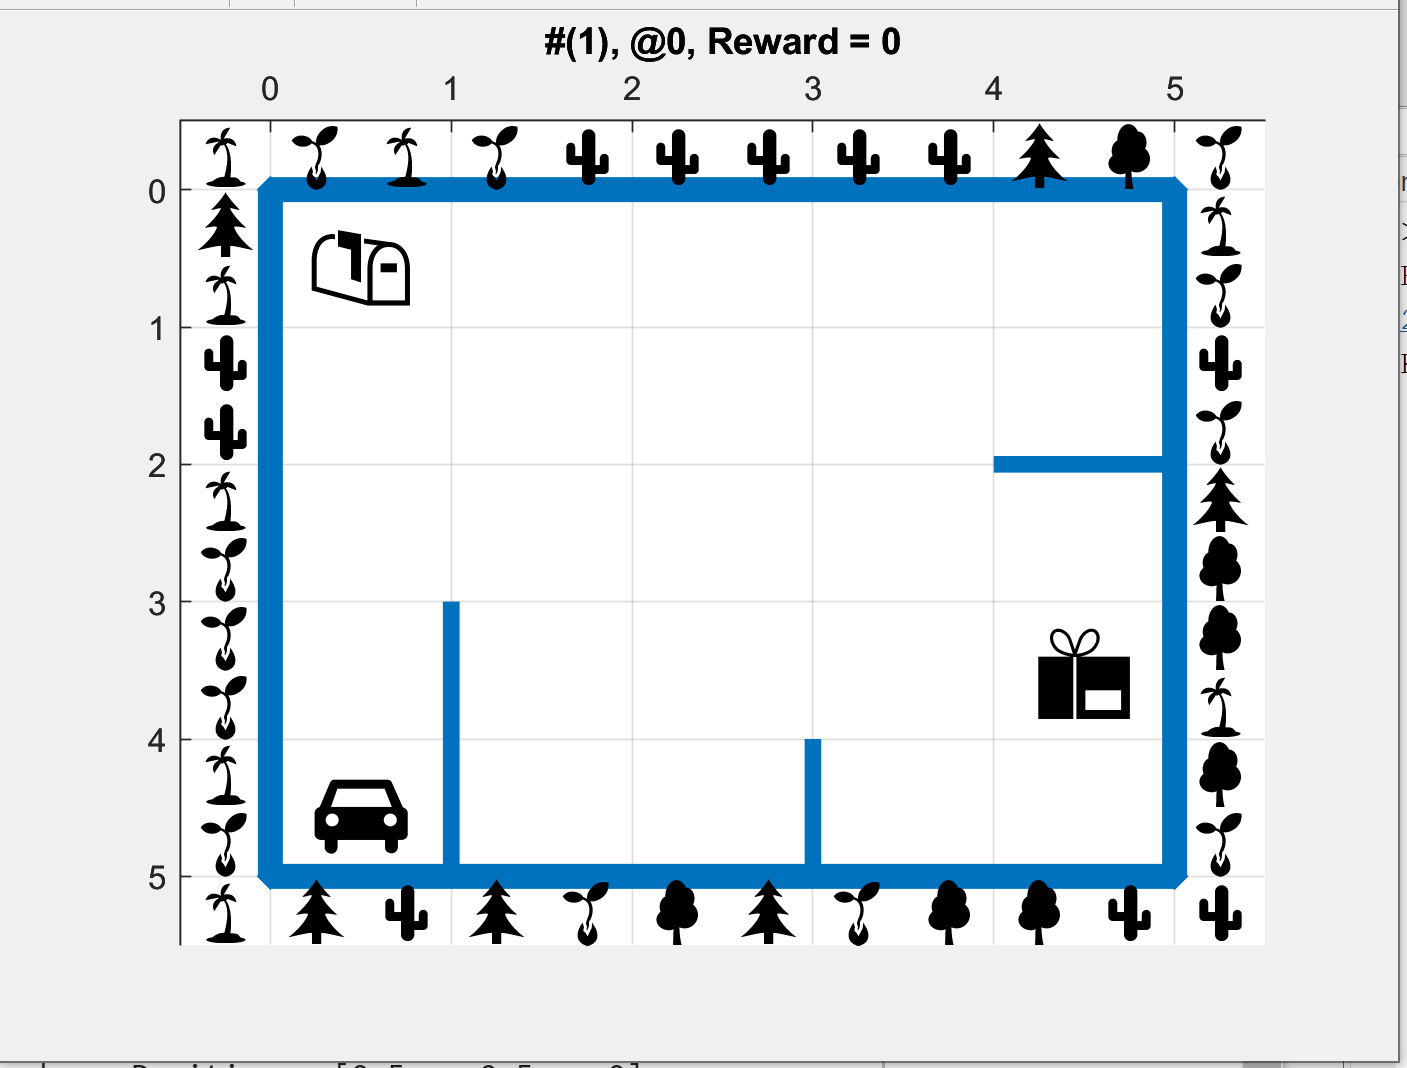
\includegraphics[width=0.45\linewidth]{pics/S0.PNG}
    }
    \hfill
    \subfloat[]{
        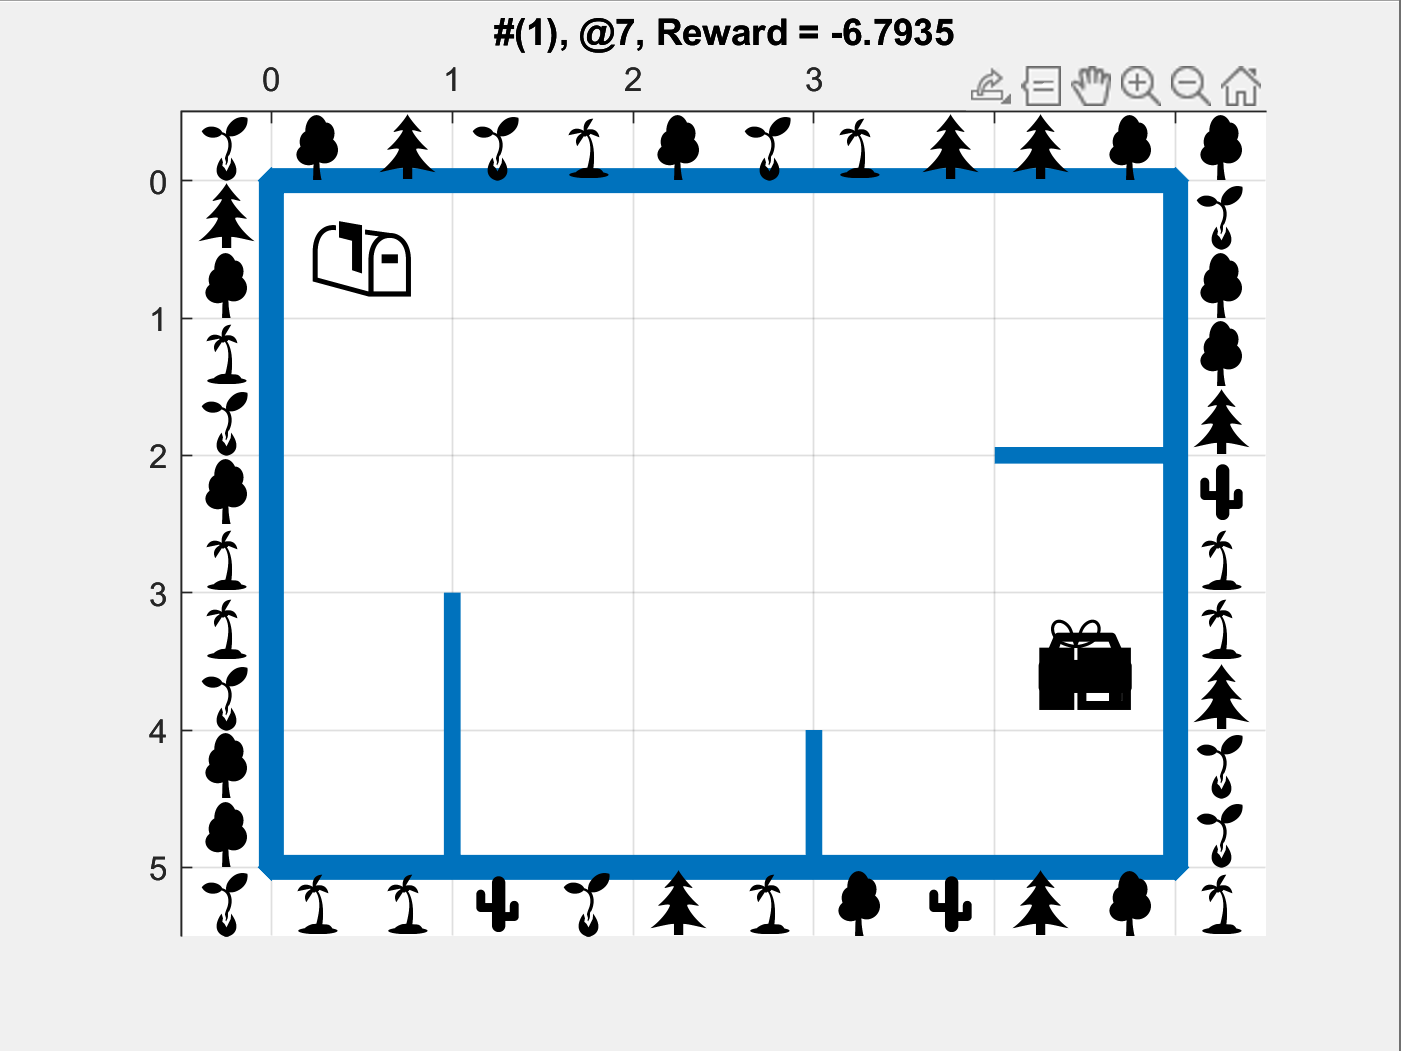
\includegraphics[width=0.45\linewidth]{pics/S1.PNG}
    }
    \hfill
    \subfloat[]{
        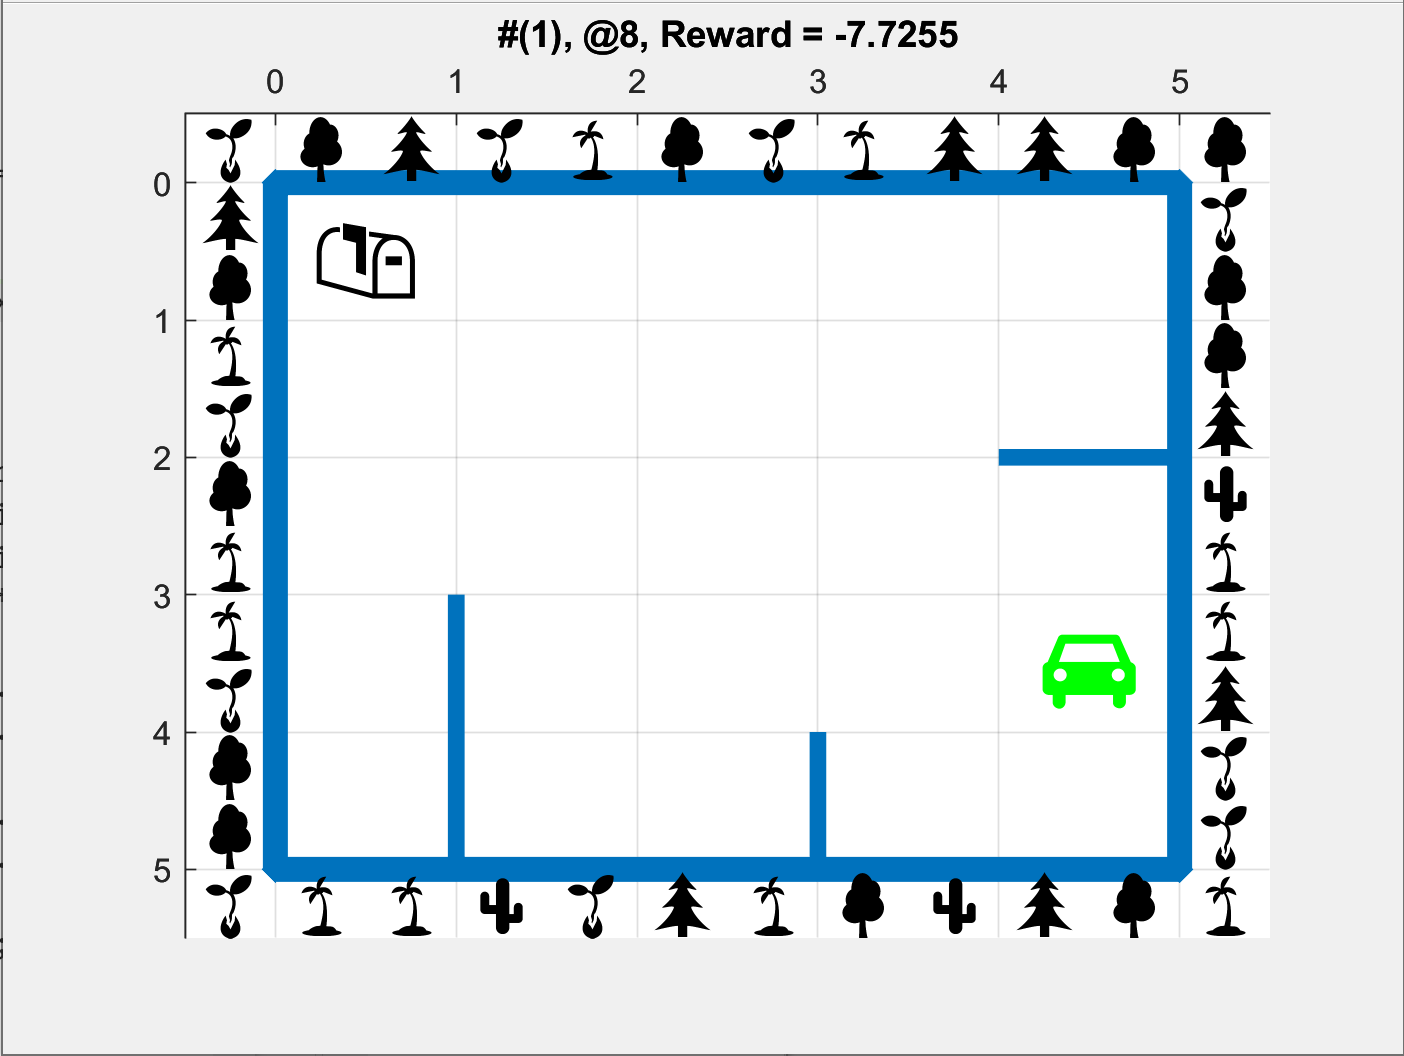
\includegraphics[width=0.45\linewidth]{pics/S2.PNG}
    }
    \hfill
    \subfloat[]{
        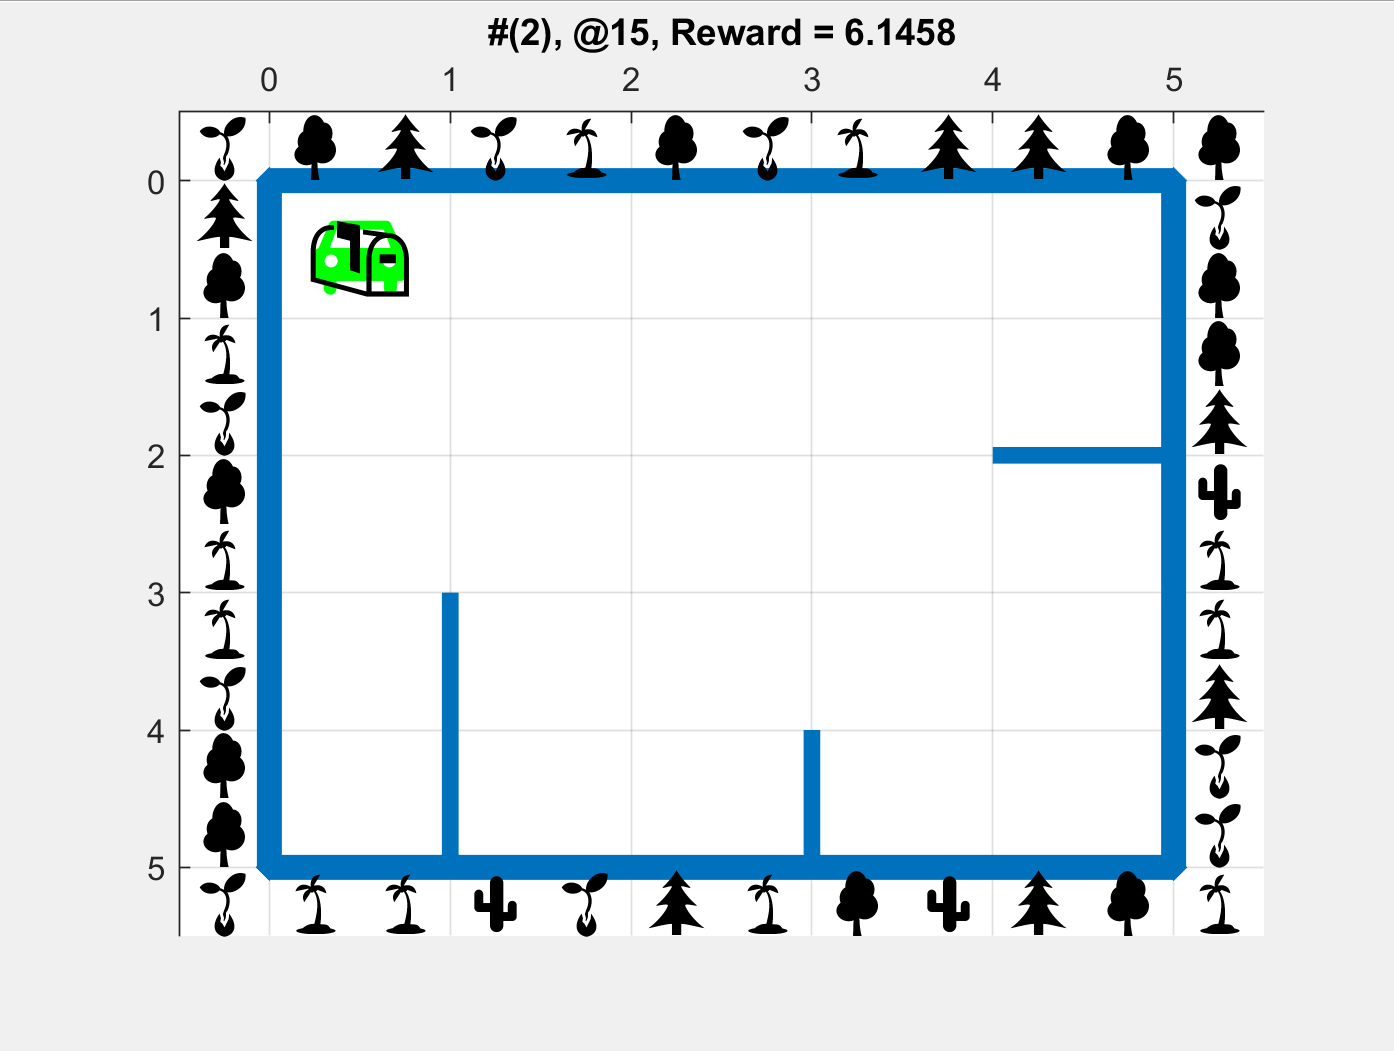
\includegraphics[width=0.45\linewidth]{pics/S3.PNG}
    }
    \caption{\centering{(a) Start Point, (b) Arriving the agent to the package location, (c) Picking the package up, (d) successfully deliver the package to the destination.}}
    \label{fig:SIM}
\end{figure*}


To retrain the agent just change the value of \textit{$load_{en}$} variable to false and run the main script. To use the pretrained network, change it back to true value and run the script.


%%%%%%%%%%%%%%%%%%%%%%%%%%%%%%%%%%%%%%%%%%%%%%%%%%%%%%%%%%%%%%%%%%%%%%%%%%%%%%%%%%
%                   Discussion
%%%%%%%%%%%%%%%%%%%%%%%%%%%%%%%%%%%%%%%%%%%%%%%%%%%%%%%%%%%%%%%%%%%%%%%%%%%%%%%%%%
\section{Discussion}
    
In this project, a post-delivery robot was successfully trained using Deep Q-Learning within a 5×5 gridworld environment. By replacing the traditional tabular Q-learning approach with a neural network–based function approximator, the agent was able to efficiently handle the large state space of 500 distinct states. The use of an experience replay buffer, a target network, and an $\epsilon$-greedy policy enabled stable learning and effective convergence.

The trained policy demonstrated near-optimal behavior, reliably guiding the robot to pick up the package and deliver it to the designated destination while minimizing illegal moves and unnecessary steps. Simulation results and policy visualizations confirmed that the learned strategy generalized well across different package and destination configurations.

Overall, the findings highlight the potential of deep reinforcement learning techniques such as DQN for solving navigation and delivery problems with discrete actions and sparse rewards. Future work could extend this framework to larger gridworlds, continuous environments, or real-world robotic systems, as well as explore more advanced algorithms like Double DQN or Dueling DQN for improved stability and performance.







\end{document}


